\Chapter{Processz ütemezés}

\Section{Az ütemezési probléma}
%TODO referencia könyvből: Mastering Linux Kernel Development: A kernel developer's reference manual

Minden operációs rendszer hatékonysága arányos azzal a képességével, amely a processzek fair ütemezését végzi. A processz ütemező, a kernel központi eleme, ő az aki eldönti hogy mikor és mennyi időre bírtokolhatja egy folyamat a processzort. Ideális esetben, a processzeknek időszeletekre van szükségük a futáshoz,az ütemezőknek lényegében a processzor időszeleteit kell tisztességesen felosztaniuk a folyamatok között.
Egy ütemező algoritmusnak ki kell elégitenie, néhány kritériumot:
\begin{itemize}
	\item Pártatlanság: minden folyamat (processz, taszk, job) korrekt módon (nem feltétlenül egyenrangúan) kapjon CPU-t.
	\item Hatékonyság: a CPU lehetőleg a legnagyobb százalékban legyen kihasználva.
	\item Válaszidő: az interaktív felhasználóknak a válaszidőt minimalizálják, (ne vesszék el türelmüket, hiszen a "vakon" nyomogatott gombok tovább lassíthatnak).
	\item Fordulási idő(turnaround time): a kötegelt munkák (job) fordulási idejét minimalizálni
kell.
	\item Teljesítmény: az időegységre eső job-feldolgozás, interaktív munka maximalizálása.
(Lássuk be, ez különbözik a fent említett hatékonyságtól.)
\end{itemize}
Láthatók bizonyos ellentmondások a kritériumok között. A válaszidő minimalizálása eredményezheti a fordulási idő növekedését!
A számításigényes munkák korlátozás nélküli
előnyben részesítése javítja a hatékonyságot, de nem biztosítja a korrektséget, és az összevont
teljesítmény is csorbulhat.
Jelenleg a kernel 5.8.x verziójában, a normál processzek ütemezését a CFS ütemezési osztály végzi. 

\Section{Elterjedt ütemezési stratégiák}

\SubSection{$\mathcal{O}(n)$}
Az $O(n)$ ütemező, amelyet a Linux kernelben használtak 2.4 és 2.6 verziók között. A müködési elve egyszerűnek mondható, mivel végigiterál az összes futásra kész állapotú processzen, és megválasztja a legmagasabb prioritási értékkel rendelkezőt.
Ez egy $O(n)$ műveletigényű algoritmus volt, ahol az $n$ a futtatható processzek számát jelölte. Emiatt nagy processzámnál nem volt elég effektív és a valós idejű processzek így kiszámíthatlanok lettek.
Egy runqueue-t használt, hogyha a processzek száma kevesebb volt mint a processzormagok száma, a maradék processzor egy "tétlen" állapotba került. Emiatt ez az ütemező nem volt túl hatékony erőforrás kihasználásban sem.
%TODO referencia: http://www.cse.iitm.ac.in/~chester/courses/16o_os/slides/7_Scheduling.pdf
%TODO referencia: https://www.programmersought.com/article/71614915531/

\SubSection{$\mathcal{O}(1)$}
Az $O(n)$ ütemező különféle problémái miatt, leváltotta az $O(1)$ ütemező, amit a Linux kernel 2.6 verziójától, 2.6.22 verzióig használták. 
Konstans idő alatt választott következő processzt futásra, emiatt nagy processz szám mellett is használható volt.
A folyamatokat, két részre osztja, Real-time illetve normál processzekre. A valós idejű processzek 0-99-ig kapnak prioritási szinteket, amíg a normál processzek(Batch vagy interactive) 100-139-ig. Itt a 100-as prioritás jelöli a legfontosabb processzt, amíg a 139 a legkevésbé fontosat. Normál processzekhez egy alapértelmezett 120-as statikus prioritást rendeltek. 
%TODO referencia: http://www.cse.iitm.ac.in/~chester/courses/16o_os/slides/7_Scheduling.pdf
%TODO referencia: https://www.researchgate.net/publication/4376448_Fairness_and_interactive_performance_of_O1_and_CFS_Linux_kernel_schedulers

Processzoronként, két listát tart nyilván amiben tárolódnak a futásra kész processzek. (Active run queue, Expired run queue)

\begin{figure}[h]
\centering
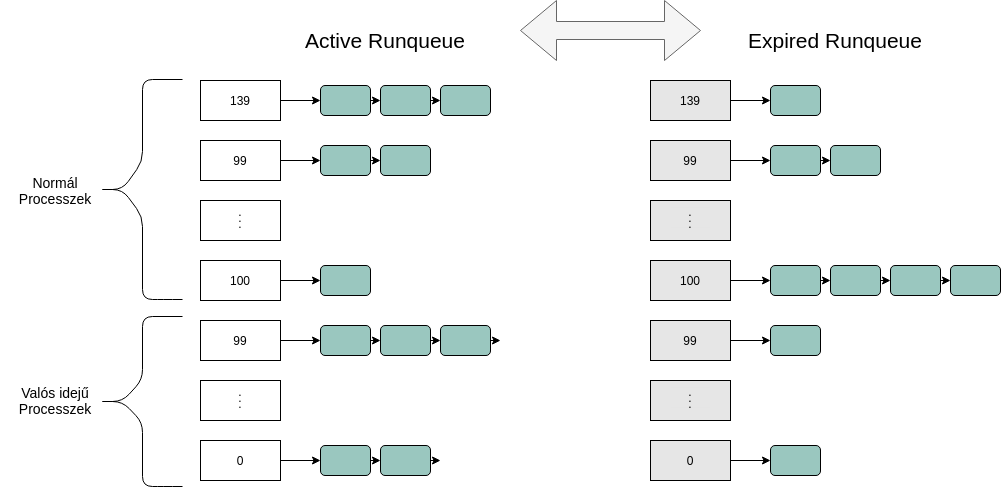
\includegraphics[width=\textwidth]{images/activeExpiredRunqueue.png}
\caption{Active and Expired Run queues}
\label{fig:Active and expired runqueues}
\end{figure}

%TODO referencia könyvből:Understanding the Linux Kernel, Third Edition 259

Mindig az aktív listából választja ki a legfontosabb processzt futásra. Miután futott egy időszeletnyit, ez a processz, átkerül az expired run queue-ba, egy új dinamikusan számolt prioritással.
Emiatt ahogy haladunk előre az időben az active run queue-ból folyamatosan fogynak el a processzek.  Amikor az active run queue végzett a processzekkel, a két lista felcserélődik és folyatatódik a végrehajtás az új listával.
Annak érdekében hogy meglehessen különböztetni a batch és az interactive processzeket, egy úgynevezett "bonus" valtozót tartunk nyilván, ami a dinamikus prioritás számításnál fog előkerülni. Ennek az értéke 0 és 10 között mozoghat.
\begin{cpp}
dynamic priority = MAX(100, MIN(static priority - bonus + 5, 139))
\end{cpp}
Amikor a bonus változó értéke kisebb mint 5, arra utal hogy kevesebb interakciót fog végezni a felhasználóval, így több cpu lázas szakasza lesz a processznek élete során. Ilyenek tipikusan a batch processzek.
Ha a bonus változó értéke nagyobb mint 5 lesz, valószínűleg a processz élete során sok interakció fog végezni a felhasználóval. Ez inkább az interactive processzekre jellemző.

\noindent\textit{Batch Process} 

\setlength{\leftskip}{1cm}

\noindent Nem igényelnek felhasználóval történő interakciót, általában a háttérben futnak. Ezeknek a processzeknek nincs szükségük arra hogy reszponzívak legyenek, tipikusan ilyenek a programozási nyevlek fordítói, adatbázis motorok és tudományos számítások.

\setlength{\leftskip}{0pt}

\noindent\textit{Interactive Process}

\setlength{\leftskip}{1cm}

\noindent Folytonos interakciót igényelnek a felhasználóval, az életidejük nagy részét gomb leütésekre és egér mozdulatokra történő várakozással tölti.
Amikor az input beérkezik, gyorsan reagálniuk kell, ellenkező esetben a felhasználó lassúnak fogja találni a rendszert és ezt el szeretnénk kerülni.
Az interactive processzek általában nem fejezik be az időszeletüket amit kapnak, ezért nekik nagyobb időszeletet kell biztosítani. 

\setlength{\leftskip}{0pt}

Az időszelet meghatározása úgy történik, hogy amelyik processz kevesebb mint 120-as prioritással rendelkezik, nagyobb időszeletet kap, 120-nál nagyobb prioritású processzek pedig kevesebbet.
\begin{cpp}
if priority < 120 
	time slice = (140 - priority) * 20    milliseconds 
else
	time slice = (140 - priority) * 5   milliseconds 
\end{cpp}


%TODO referencia: http://www.cse.iitm.ac.in/~chester/courses/16o_os/slides/7_Scheduling.pdf
%TODO referencia: https://doc.opensuse.org/documentation/leap/tuning/html/book-sle-tuning/cha-tuning-taskscheduler.html#sec-tuning-taskscheduler-cfs
%TODO referencia: https://elixir.bootlin.com/linux/v5.8.5/source/kernel/sched/fair.c
%TODO referencia: https://www.researchgate.net/publication/4376448_Fairness_and_interactive_performance_of_O1_and_CFS_Linux_kernel_schedulers
%TODO referencia könyvből: Linux Kernel Development 3rd Edition 51.oldal
\Section{A linux ütemező felépítése}

A linux operációs rendszer elsődlegesen asztali gépekhez lett tervezve, ennek ellenére hamar multi-dimenziós operációs rendszerré nőtte ki magát, széles körben használták beágyazott rendszerek, mainframe-eken, szuperszámítógépeken és szoba méretű szervereken is. Különböző platformok is befogadták, mint például valós idejű rendszerek, SMP, virtualizáció. Az ilyen változatos platformok miatt, alakultak ki a típusai a processzeknek. Egy asztali rendszeren, többnyire magas interaktivitású processzeket kell ütemezni, amik I/O igényesek, a valós idejű rendszereken pedig inkább  determinisztikus processzek jellemzőbbek. A különböző típusú processzeket, egymástól eltérő heurisztikus módszerekkel ütemezhetjük fair módon.

\SubSection{Ütemezési osztályok}
A linux ütemező moduláris, emiatt lehetővé teszi hogy különböző algoritmusok ütemezzenek, különböző típusú processzeket. Ezt a modularitást, ütemező osztályoknak nevezzük. Belső kialakitássa igen ügyesen kezeli a különböző processz típusokat, egy két rétegű modelt használ. Az első réteg egy Generic Scheduler(általános ütemező), ami absztrakt műveleteket határoz meg, ez egy belépési függvény az ütemező számára. A második réteg maga az ütemező osztály, amiben a tényleges ütemezési műveleteket tartalmazza, itt történik a különböző  processz osztályok ütemezése.

\begin{figure}[h]
\centering
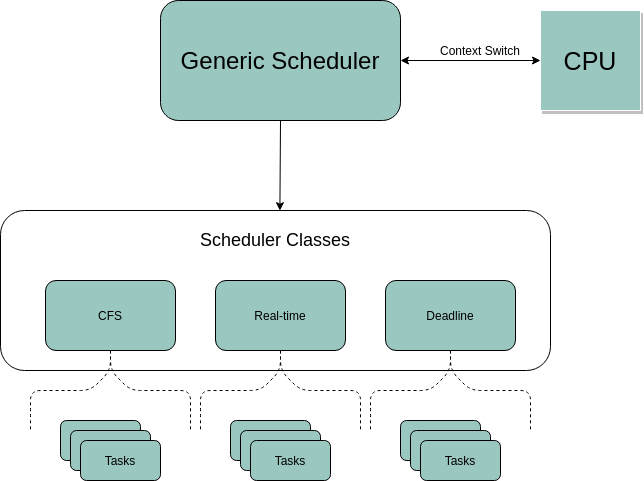
\includegraphics[scale=0.4]{images/genericScheduler.png}
\caption{Generic Sheduler and Scheduler Classes}
\label{fig:Generic Sheduler and Scheduler Classes}
\end{figure}

Ez a modell lehetővé teszi, hogy az Generic Scheduler elvont maradjon minden ütemező osztály megvalósítási részleteitől. Így a normál processzek ütemezéséért, az egyik ütemező osztály felel, amíg determinisztikus végrehajtást igénylő processzekért, mint a valós idejű folyamatok, egy másik osztály. Ez az architechtúra lehetővé teszi azt is hogy, akár új ütemező osztályt vezessünk be.

A Generic Scheduler egy absztrakt interface-t definiál a sched\_class struktúrán keresztül:
%TODO referencia: https://elixir.bootlin.com/linux/v5.8.5/source/kernel/sched/sched.h#L1743
\begin{cpp}
struct sched_class {
	const struct sched_class *next;

#ifdef CONFIG_UCLAMP_TASK
	int uclamp_enabled;
#endif

	void (*enqueue_task)
		(struct rq *rq, struct task_struct *p, int flags);
	void (*dequeue_task)
		(struct rq *rq, struct task_struct *p, int flags);
	void (*yield_task)   (struct rq *rq);
	bool (*yield_to_task)
		(struct rq *rq, struct task_struct *p, bool preempt);

	void (*check_preempt_curr)
		(struct rq *rq, struct task_struct *p, int flags);

	struct task_struct *(*pick_next_task)(struct rq *rq);

	void (*put_prev_task)(struct rq *rq, struct task_struct *p);
	void (*set_next_task)
		(struct rq *rq, struct task_struct *p, bool first);

#ifdef CONFIG_SMP
	int (*balance)
	  (struct rq *rq, struct task_struct *prev, struct rq_flags *rf);
	int  (*select_task_rq)
	  (struct task_struct *p, int task_cpu, int sd_flag, int flags);
	void (*migrate_task_rq)(struct task_struct *p, int new_cpu);

	void (*task_woken)(struct rq *this_rq, struct task_struct *task);

	void (*set_cpus_allowed)(struct task_struct *p,
				 const struct cpumask *newmask);

	void (*rq_online)(struct rq *rq);
	void (*rq_offline)(struct rq *rq);
#endif

	void (*task_tick)
		(struct rq *rq, struct task_struct *p, int queued);
	void (*task_fork)(struct task_struct *p);
	void (*task_dead)(struct task_struct *p);

	/*
	 * The switched_from() call is allowed to drop rq->lock, 
	 * therefore we
	 * cannot assume the switched_from/switched_to 
	 * pair is serliazed by
	 * rq->lock. They are however serialized by p->pi_lock.
	 */
	void (*switched_from)
		(struct rq *this_rq, struct task_struct *task);
	void (*switched_to) 
		(struct rq *this_rq, struct task_struct *task);
	void (*prio_changed)
		(struct rq *this_rq, struct task_struct *task,
			      int oldprio);

	unsigned int (*get_rr_interval)(struct rq *rq,
					struct task_struct *task);

	void (*update_curr)(struct rq *rq);

#define TASK_SET_GROUP		0
#define TASK_MOVE_GROUP		1

#ifdef CONFIG_FAIR_GROUP_SCHED
	void (*task_change_group)(struct task_struct *p, int type);
#endif
};

\end{cpp}
 
Minden ütemező osztálynak prioritása van. 
Az általános ütemező, végigiterál az ütemező osztályokon és azt a legnagyobb prioritással rendelkező osztályt fogja választani, amiben található futtatható processz. A megválasztott ütemezési osztály fogja eldönteni hogy melyik processz kerülhet végrehajtásra.

A kernel 5.8.x verziójában, három ütemezési osztály található, ezek névszerint: 
\begin{itemize}
	 \item Completely Fair Scheduler class
	 \item Real-time class
	 \item Deadline class
\end{itemize}
A következő kódrészletek megmutatják, külön-külön az osztályok hogyan definálják a sched\_class absztrakt struktúrát.

%TODO referencia: https://elixir.bootlin.com/linux/v5.8.5/source/kernel/sched/fair.c#L11126
Completely Fair Scheduler class(/kernel/sched/fair.c):
\begin{cpp}
const struct sched_class fair_sched_class = {
	.next			= &idle_sched_class,
	.enqueue_task		= enqueue_task_fair,
	.dequeue_task		= dequeue_task_fair,
	.yield_task		= yield_task_fair,
	.yield_to_task		= yield_to_task_fair,

	.check_preempt_curr	= check_preempt_wakeup,

	.pick_next_task		= __pick_next_task_fair,
	.put_prev_task		= put_prev_task_fair,
	.set_next_task          = set_next_task_fair,
...
};
\end{cpp}

%TODO referencia: https://elixir.bootlin.com/linux/v5.8.5/source/kernel/sched/rt.c#L24321
Real-time Scheduler class(/kernel/sched/rt.c):
\begin{cpp}
const struct sched_class rt_sched_class = {
	.next			= &fair_sched_class,
	.enqueue_task		= enqueue_task_rt,
	.dequeue_task		= dequeue_task_rt,
	.yield_task		= yield_task_rt,

	.check_preempt_curr	= check_preempt_curr_rt,

	.pick_next_task		= pick_next_task_rt,
	.put_prev_task		= put_prev_task_rt,
	.set_next_task          = set_next_task_rt,
...
};
\end{cpp}

%TODO referencia: https://elixir.bootlin.com/linux/v5.8.5/source/kernel/sched/deadline.c#L2433
Deadline Scheduler class(/kernel/sched/deadline.c):
\begin{cpp}
const struct sched_class dl_sched_class = {
	.next			= &rt_sched_class,
	.enqueue_task		= enqueue_task_dl,
	.dequeue_task		= dequeue_task_dl,
	.yield_task		= yield_task_dl,

	.check_preempt_curr	= check_preempt_curr_dl,

	.pick_next_task		= pick_next_task_dl,
	.put_prev_task		= put_prev_task_dl,
	.set_next_task		= set_next_task_dl,
...
};
\end{cpp}

%referencia: https://www.kernel.org/doc/html/latest/scheduler/sched-design-CFS.html

\SubSection{Ütemezési politikák(Scheduling policy)}

A CFS osztály három ütemezési politikát implementál
\begin{itemize}
	\item SCHED\_OTHER(tradicionálisan  SCHED\_NORMAL) - Alapértelmezett ütemezési algoritmus, amit a normál processzek nagytöbbsége is használ.

    \item SCHED\_BATCH - Közel sem hajt végre olyan sok preempciót mint az átlagos taszkok, ezáltal lehetővé téve azt hogy a taszkok tovább fussanak, de ennek az ára az interaktivitás csökkenése.
        
	\item SCHED\_IDLE - Ezt az ütemezési politikát, kis intenzitású processzek esetén használják. Ezzel még a nice $+19$-től kisebb prioritást szabhatunk a processzünknek.
\end{itemize}
A valós idejű ütemezési osztály implementálja a SCHED\_FIFO és SCHED\_RR politikákat, ezek a POSIX által lettek meghatározva.
\begin{itemize}
	\item SCHED\_FIFO - Időkritikus, valós idejű processzek ütemezésénél használják. A nevében is benne van, FIFO jellegű azaz First-In First-out, az elsőnek érzekett processz kerül először kiszolgálásra. 

	\item SCHED\_RR - SCHED\_FIFO-hez hasonló, szintén valós idejű processzekhez használják. A Kerge Rigó ütemezési algoritmust használja.
\end{itemize}

A SCHED\_DEADLINE politika, a sched\_dl ütemezési osztályban található.  Earliest Deadline First (EDF) ütemezési algoritmus implementációja.

\SubSection{Runqueues}

Hagyományosan a runqueue, az az adatstruktúra ami tárolja az összes processzt, akik a cpu-ért versenyeznek.
Minden processzor maghoz, külön runqueue tartozik. 
Az Generic Scheduler réteg egy absztrakt runqueue-t implementál, olyan elemekkel amik egy runqueue interface-nek felelnek meg.
Ez a struktura ki lett bővítve néhány pointerrel, amik a különböző osztályok futási soraikra mutatnak. Ez azt jelenti hogy a különböző ütemezési osztályok futási soraik, mind bele vannak ágyazva a fő runqueue struktúrába. Ezáltal minden ütemező osztálynak lehetősége van megválasztani, a saját runqueue adat struktúráját. 


\SubSection{Processz Prioritási szintek és azok módosítása}

Annak az eldöntése hogy melyik processz kerül legközelebb végrehajtásra, függ a prioritástól. Minden processz el van látva egy prioritás értékkel ami lehet dinamikus prioritás vagy statikus prioritás.

Dinamikus prioritásnak nevezzük azt amit a kernel normál folyamatoknál alkalmaz. Ehhez az értékhez figyelembe veszi a processz nice értékét, az elmúlt időben megfigyelt tevékenységét (CPU vagy I/O lázas processz) és hogy mennyi időt töltött várakozással, illetve  végrehajtással.
A normál processzekhez alapértelmezett prioritását meg tudjuk változtatni a nice, illetve a renice paranccsal.

\begin{python}
$ nice -n N ./a.out 
\end{python}%$


Ahol az N értéke +19 és -20 között mozoghat.
Nagyobb nice érték azt jelzi hogy mennyire vagyunk "nagylelkűek" a többi programhoz, azáltal hogy őket előre engedjük.

A processzek nice értékeiket lekérdezhetjük a ps programmal.
\begin{python}
$ ps -Al
\end{python}%$


Statikus prioritást valós idejű processzeknél alkalmazzák. Ilyen prioritást felhasználó is adhat processznek, ekkor a kernel nem módosíthatja dinamikusan az értéket.
A statikus prioritású processzek tehát, elsőbbséget élveznek ütemezéskor.
Egy processz statikus prioritási értéke, pedig adott ütemezési politikákhoz mérten változhat. Ezeket a \texttt{chrt -m} paranccsal láthatjuk.
\begin{python}
$ chrt -m
SCHED_OTHER min/max priority	: 0/0
SCHED_FIFO min/max priority	: 1/99
SCHED_RR min/max priority	: 1/99
SCHED_BATCH min/max priority	: 0/0
SCHED_IDLE min/max priority	: 0/0
SCHED_DEADLINE min/max priority	: 0/0
\end{python}%$


A linux kernel szemszögéből, a processz prioritásokat skálázása 0-tól, 139-ig történik. A valós idejű processzek 0-tól 99-ig kapnak prioritást, amíg a normál folyamatok pedig 100-tól, 139-ig.


Normál processzek esetén 120-as a statikus prioritás, ezt az értéket módosíthatjuk, a nice illetve a renice-paranccsal.
Ez a nice érték -20 és +19 között mozoghat, attól függően hogy mennyire szeretnénk nagylelkűek lenni, a többi processzel szemben.

A processzeknek lekérdezhetjük, illetve megváltoztathatjuk az ütemezési politikáikat szintén a chrt program segítségével. A példánkban a processzünk pidje 31475.

\noindent Az ütemezési polika lekérdezése:
\begin{python}
$ chrt -p 31475
pid 31475 current scheduling policy: SCHED_OTHER
pid 31475 current scheduling priority: 0
\end{python}%$

\noindent A processz ütemezési politikájának megváltozatása:
\begin{python}
$ chrt -rr -p 99 31475
$ chrt -p 31475
pid 31475 current scheduling policy: SCHED_RR
pid 31475 current scheduling priority: 99
\end{python}%$

Real-time processzek esetén, a prioritási szinteik ellentétesek a normál processzekéhez képest. A legfontosabb prioritási szint a 99-es és a legkevésbé fontos pedig az 1-es.
%TODO referencia: https://access.redhat.com/solutions/3742421
DeadLine processzek is ugyanilyen egyszerűen készíthetők a chrt programmal.
Itt viszont ki kell bővítenünk három paraméterrel a programunkat.
\begin{itemize}
\item Runtime: A feladatra kijelölt végrehajtási idő.
\item Deadline: A periódus megkezdése után milyen gyorsan kell elindítani a futási időt
\item Period:  Milyen gyakran hajtják végre a futási időt
\end{itemize}
A kernel megköveteli, hogy a következők igazak legyenek:
\begin{equation}
RUNTIME <= DEADLINE <= PERIOD
\end{equation}
Bármelyik paraméter elhagyása az alábbiakat eredményezi.
\begin{itemize}
\item A futásidő elhagyása azt eredményezi hogy, futási időt a határidő értékére állítja.
\item A határidő elmulasztása azt eredményezi, hogy a határidőt a periódus értékére kell beállítani.
\item A periódus elmulasztása a periódust, a határidő értékére kell állítani.
\end{itemize}
\noindent Ezzel a három plusz paraméterrel, így néz ki a chrt program paraméterezése:
\begin{python} 
$ sudo chrt -d --sched-runtime 1000000 --sched-deadline 5000000 
		--sched-period 5000000 0 ./test
\end{python}%$

\SubSection{Completely Fair Scheduler}


A Completely Fair Scheduler azaz a CFS, váltotta le a korábbi $O(1)$ -s ütemezőt a linux kernel 2.6.23 verzióban.
Az összes dinamikus prioritású folyamatot a CFS osztály kezeli. Általános célú Unix rendszerekben, normál processzekből fordul elő a legtöbb, ebből is következik hogy a CFS ütemező osztály a legelfoglaltabb.
A CFS nem támaszkodik a hagyományos időszeletekre a processzor kiosztásakor, hanem inkább a virtuális futásidő (vruntime) fogalmát vezeti be.
A vruntime változó tárolja el a virtuális futás idejét egy processznek, ami igazából a tényleges futási idő normálizálva, a futtatható processzek darabszámával.
A virtual runtime mértékegysége a nanoszekundum. (1 nanoszekundum = $\frac{1}{1,000,000,000}$ másodperc)
A virtual runtime segítségével szeretnénk megközelíteni az ideális multitasking processzort, amit a CFS próbál modellezni. Egy egyszerű szabályt követ az algoritmus ami pedig az hogy, mindig válassza a legkisebb vruntime-al rendelkező taszkot. A CFS egy piros-fekete fát használ, a listában lévő futtatható taskok kezelésére és hogy egyszerűen megtalálhassa a legkisebb vruntime-mal rendelkező taskot.
A piros-fekete fa, amelyet Linux alatt rbtree-nek hívnak, egy saját magát kiegyensúlyozó bináris fa.
A fában a csomópontok egy-egy futásra kész taszkot reprezentálnak. A taszkok elhelyezkedése a fában a virtuális futásidejükhöz mérten történik. 
A fa bal oldalában helyezkednek el a kisebb vruntime-mal rendelkező taszkok.
A balszélső csomópontban mindig az a taszk található amelyik a legkevesebb a vruntime-mal rendelkezik.
\begin{figure}[h]
\centering
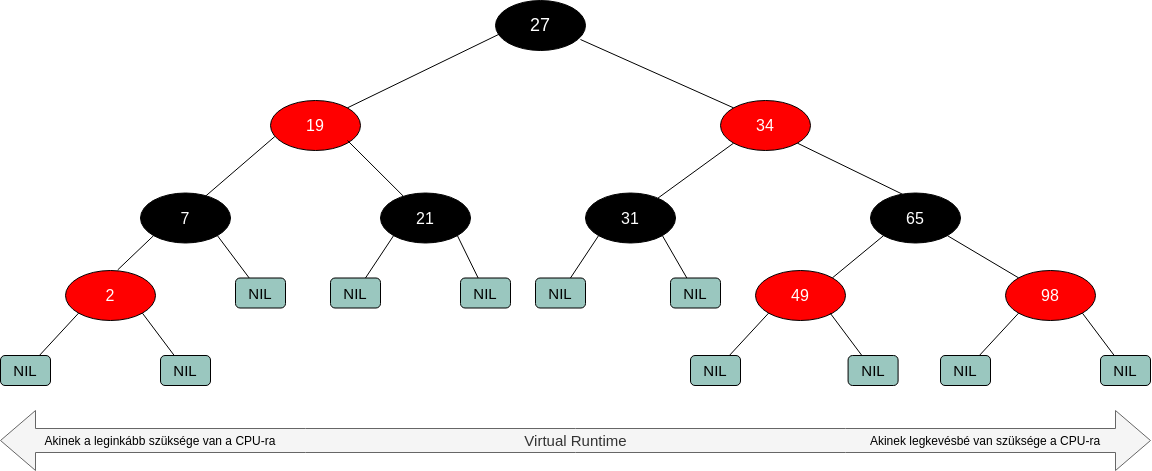
\includegraphics[width=\textwidth]{images/redBlackTree.png}
\caption{Piros fekete fa a processz prioritás értékekkel}
\label{fig:rb_tree}
\end{figure}

\noindent A piros-fekete fák önkiegyensúlyozók maradnak azáltal hogy, betartanak öt tulajdonságot:

\begin{enumerate}
	\item Egy csúcs vagy fekete vagy piros.
	\item A fa gyökere fekete.
	\item Egy piros csúcs mindkét leszármazottja fekete.
	\item Minden levél a fa gyökerével egyszínű. 
	\item Minden csúcsból a belőle leszármazó levelekbe vezető egyszerű utakon ugyanannyi fekete csúcsot érintünk.
\end{enumerate}

Amikor egy taszk futásra kész állapotba kerül, meghívódik a \textit{enqueue\_task\_fair()}  függvény, ami hatására bekerül a piros-fekete fába. Amint a taszk kilépett ebből az állapotból, az ütemező \textit{dequeue\_task\_fair()} segítségével eltávolítja a fából.
A következő kódrészletben látható hogy milyen függvényeket használ az ütemező a runqueue kezeléséhez.

\begin{cpp}
/*
 * All the scheduling class methods:
 */
const struct sched_class fair_sched_class = {
	.next			= &idle_sched_class,
	.enqueue_task		= enqueue_task_fair,
	.dequeue_task		= dequeue_task_fair,
	.yield_task		= yield_task_fair,
	.yield_to_task		= yield_to_task_fair,

	.check_preempt_curr	= check_preempt_wakeup,

	.pick_next_task		= __pick_next_task_fair,
	.put_prev_task		= put_prev_task_fair,
	.set_next_task          = set_next_task_fair,

#ifdef CONFIG_SMP
	.balance		= balance_fair,
	.select_task_rq		= select_task_rq_fair,
	.migrate_task_rq	= migrate_task_rq_fair,

	.rq_online		= rq_online_fair,
	.rq_offline		= rq_offline_fair,

	.task_dead		= task_dead_fair,
	.set_cpus_allowed	= set_cpus_allowed_common,
#endif

	.task_tick		= task_tick_fair,
	.task_fork		= task_fork_fair,

	.prio_changed		= prio_changed_fair,
	.switched_from		= switched_from_fair,
	.switched_to		= switched_to_fair,

	.get_rr_interval	= get_rr_interval_fair,

	.update_curr		= update_curr_fair,

#ifdef CONFIG_FAIR_GROUP_SCHED
	.task_change_group	= task_change_group_fair,
#endif

#ifdef CONFIG_UCLAMP_TASK
	.uclamp_enabled		= 1,
#endif
};
\end{cpp}

A vruntime váltózó értékének kiszámításához, a CFS nem csak a nice értéket használja fel hanem a process load weight változóját is. A nice értékben történő lépegetés egyesével felfelé, minusz 10\% CPU időszeletet fog eredményezni, és minden lépés lefelé pedig plusz 10\%-ot. 
A processz load weight változójának kiszámolásához a kernel fenttart egy tömböt amit \textit{sched\_prio\_to\_weight}-nek neveztek el. Itt megtalálható hogy melyik nice értékhez, milyen súly érték tartozik.
%TODO referencia a forráskódból: https://elixir.bootlin.com/linux/v5.8.5/source/kernel/sched/core.c#L8182
\begin{cpp}
const int sched_prio_to_weight[40] = {
 /* -20 */     88761,     71755,     56483,     46273,     36291,
 /* -15 */     29154,     23254,     18705,     14949,     11916,
 /* -10 */      9548,      7620,      6100,      4904,      3906,
 /*  -5 */      3121,      2501,      1991,      1586,      1277,
 /*   0 */      1024,       820,       655,       526,       423,
 /*   5 */       335,       272,       215,       172,       137,
 /*  10 */       110,        87,        70,        56,        45,
 /*  15 */        36,        29,        23,        18,        15,
};
\end{cpp}

\noindent Ez súly változó, a processz struktúrában \textit{struct load\_weight load}-ként szerepel

Egy processz vruntime változó értékét a futással töltött idejéből(\textit{delta\_exec}), processz súlyából(\textit{se->load}), illetve a nice értékéből (\textit{NICE\_0\_LOAD}) kapjuk meg.
\begin{equation}
vruntime += \frac{delta\_exec}{se->load}*NICE\_0\_LOAD
\end{equation}

Láthattuk hogyan történik a processzek megválasztása a CFS ütemezőben, de azt még nem hogy mennyi ideig futhatnak.
Ez az úgynevezett időszelet itt teljesen dinamikus számolódik.
A CFS próbál követni egy modelt, amiben ideális és tökéletes a multitask ütemezés. Ebben a rendszerben, minden processz, $1/n$ részét kapná a processzor erőforrásnak, ahol az $n$ a processzek számát jelöli. 
Tegyük fel hogy a van egy processzorunk és négy processzünk.
Egy általános Unix rendszerben a végrehajtása úgy történne, ennek a négy processznek hogy az A process futna 1 ms-t, miután végzett következik a B, szintén fut 1 ms-t és így tovább, egymást követően. A processzor 100\%-ban annak a processznek dolgozott, aki épp végrehajtásban volt.
Az ideális modelben a négy processz egyszerre futna 4ms-t, a processzor erőforrását pedig felosztanánk négy részre, így mindenki kapna 25\% -ot. Ilyen processzor sajnos nem létezik.

Az időszelet minden processz számára külön kalkulálódik, az alábbi képlet alapján.
\begin{equation}
slice = \frac{se->load.weight}{cfs\_rq->load.weight}*period
\end{equation}
Ahol se->load.weight az egyes processzek súlyaikat jelölik, cfs\_rq->load.weight pedig a runqueue-ban található összes task súly tényezője. A period nem egy konstans szám, ahhoz képest változik az értéke hogy mennyi task található a runqueue-ban. 
Az ütemező először megnézi hogy az alábbi, egyenelőtlenség teljesül-e:
\begin{equation}
nr\_running > \frac{sysctl\_sched\_latency}{sysctl\_sched\_min\_granularity}
\end{equation}
Ahol az nr\_running jelöli a runqueue-ban található taszkok számát. Ha ez az egyenlőtlenség nem teljesül, az ütemező tudni fogja hogy túl sok a taszk, ezért hogy mindenkinek biztosítson elegendő időt, egy bizonyos alsó határt fog felhasználni a következő képpen.
\begin{equation}
period =  nr\_running * sysctl\_sched\_min\_granularity
\end{equation}
Ez az alsó határ, az úgynevezett \textit{min\_granularity}.
Ez látható az alábbi kódrészletben is.
\begin{cpp}
static u64 __sched_period(unsigned long nr_running)
{
	if (unlikely(nr_running > sched_nr_latency))
		return nr_running * sysctl_sched_min_granularity;
	else
		return sysctl_sched_latency;
}
\end{cpp}

\SubSection{Csoportos ütemezés}

Annak érdekében hogy az ütemezés fair módon történjen, a CFS-t úgy tervezték hogy minden processz számára garantáljon legalább egy futást a processzoron egy bizonyos időn belül, amit úgy neveznek hogy ütemezési periódus.
A CFS ezt ütemezési periódus feldarabolja időszeletekre és ezeket osztjszét a taszkokhoz tartozó szálak között, így próbálja meg elkerülni a kiéhezés problémát. 
Tegyük fel hogy az A taszk tíz szálon szeretne futni és a B taszk pedig öt szálon. Ekkor a CFS kiosztja az időszeleteket a szálaknak igazságosan, ez pedig ahhoz vezet hogy, az A taszk és a hozzá tartozó szálai több időszeletet kapnak, ez pedig nem igazságos a B processzel szemben.
Ebből kifolyólag az is megtörténhet hogyha, az A processz még több szálon szeretne futni, így a B processz mindig csak minimális időszeletet fog kapni.(Ami 1 ms) Annak érdekében hogy mindenkivel szembe igazságosak legyünk, A és B processzeknek egyforma időszeletet kell adnia az ütemezőnek. Ez azt jelenti hogy A és B processz 50\%-50\% időszeleteket kapnak és ezt a részt felosztják a szálak között, tehát az A processznek mind a tíz szála külön-külön 5\%-ot fognak megkapni.
Annak érdekében hogy, ezt az igazságtalan időszelet kiosztást elkerüljük, a CFS csoportos ütemezést használ. Itt konkrétan a csoport kapja meg a processzor időt, és nem a szálak külön-külön.
A CFS taszk csoportok, a sched\_entity strúktúra egy része, és minden csoport megfeleltethető egy ütemezési entitásnak.

\begin{figure}[h!]
\centering
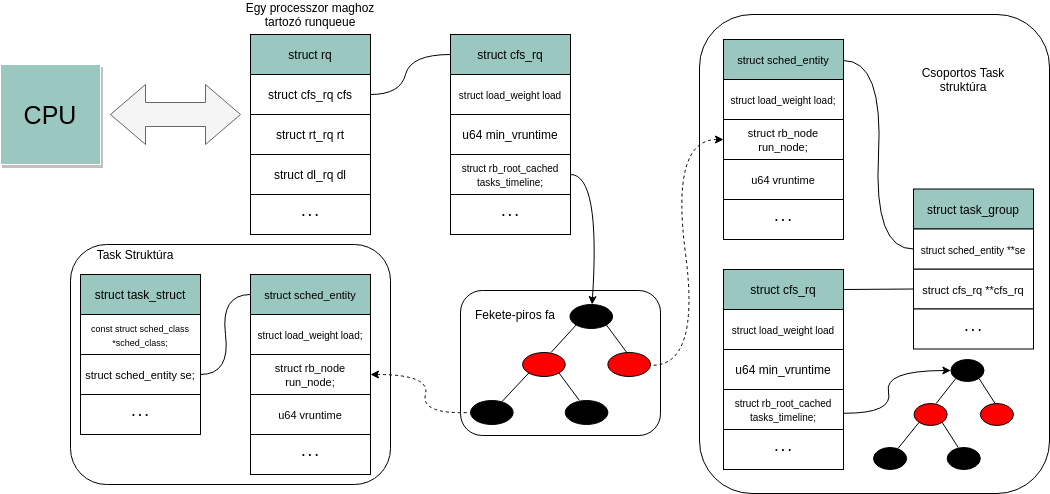
\includegraphics[width=\textwidth]{images/structureHierarchy.png}
\caption{Struktúra hierarchia}
\label{fig:structurehierarchi}
\end{figure}

\Section{Kernel modulok}
%TODO referencia könyvből: The Linux Kernel Module Programming Guide. Peter Jay Salzman Michael Burian Ori Pomerantz. Copyright © 2001 Peter Jay Salzman.  
%TODO referencia könyvből: Understanding the Linux Kernel, Third Edition by Daniel P. Bovet and Marco Cesati
Egy modul gyakorlatilag instrukciók sorozata, amit igény szerint, ki és be lehet tölteni a kernel-be. Kibővíti a kernel funkcionalitását, anélkül hogy újra keljen indítani a rendszert. Minden magasabb szintű kernel komponens, mint például fájlrendszerek, I/O eszköz driver, hálózati rétegek, stb, meg lehet írni modulként és be lehet tölteni a kernel-be.

\noindent Az éppen aktuálisan betöltött moduljainkat, le tudjuk kérdezni az \texttt{\# lsmod} paranccsal, ami a \texttt{/proc/modules} fájl tartalmát listázza.

A modulok ELF objektumként tárolódnak a fájlrendszeren, amik a kernelhez vannak linkelve, ezt a linkelést az \texttt{\# insmod} paranccsal tudjuk elvégezni.
A modulok egy duplán láncolt listában tárolódnak.
Ha ebből a listából el szeretnénk távolítani egy modult(unlink), az \texttt{\# rmmod} programot használhatjuk, ami a következő műveleteket végzi el:
\begin{enumerate}
	\item Beolvassa a parancssorból annak a modulnak a nevét, amit el kívánunk távolítani.
	\item Megnyitja a \texttt{/proc/modules} fájlt és leellenőrzi hogy a modul, ténylegesen linkelve van-e a listába.
	\item Meghívja a \texttt{delete\_modul()} rendszerhívást és továbbadja neki a modul nevét.
	\item Terminálódik.
\end{enumerate} 

Minden kernel modulnak kell hogy legyen legalább két eljárása, az egyik ilyen \texttt{init\_module()}.
Ez egy inicializációs eljárás, az \texttt{init\_module()} hívódik meg amikor beszúrjuk a modult az \texttt{insmod} paranccsal.
A másik a \texttt{cleanup\_module()}, ami pedig az eltávolítás során(\texttt{rmmod}) hívódik meg.
A 2.3.13.-as kernel verzióban bevezettek egy újítást, ami szerint, mi határozhatjuk meg az eljárások neveit. Ehhez használjuk a \texttt{module\_init()} és a \texttt{module\_exit()} makrókat. Tipikusan, az \texttt{init\_module()}-ban írjuk meg a programunkat, ami lehet hogy kicserél egy kernel függvényt a miénkre vagy regisztrál valamilyen kezelőt a kernel-hez. A \texttt{cleanup\_module()}-nak pedig az lenne a feladata, hogy visszavonja a módosításokat, amit az \texttt{init\_module()} elvégzett.
%TODO referencia: https://www.kernel.org/doc/htmldocs/kernel-hacking/routines-init-again.html

A prink() függvénynek, nem a felhasználóval történő kommunikáció a fő szerepe, mégha én a mostani példában arra is használom. Ez egy naplózási eszköz(log) a kernel számára, amivel valamilyen fontos információt vagy hibaüzenetet továbbít. Az üzeneteknek, különböző fontossági szintjük van. Ezeket a szinteket hívjuk console\_loglevel-nek, ami egy kernelbeli változó, aminek a szintjeit 0-7 ig fogjuk megnézni. 
%TODO referencia: https://www.kernel.org/doc/html/latest/core-api/printk-basics.html
\begin{enumerate}
\setcounter{enumi}{-1}
	\item KERN\_EMERG \- A rendszerünk már használhatatlan állapotba került.
	\item KERN\_ALERT \- Az adódott problémákról, gondoskodnunk kell.
	\item KERN\_CRIT \- Kritikus események jelentkeztek.
	\item KERN\_ERR \- Nem kritikus hibák jelzése.
	\item KERN\_WARNING	\- Figyelmeztetések, amikre oda kell figyeljünk.
	\item KERN\_NOTICE \- Normális, általános események
	\item KERN\_INFO \- Információ továbbítás ami nem igényel beavatkozást.
	\item KERN\_DEBUG \- Kernelbeli hibakiíratás, egy kimenet a kernel oldalról, hogyha a fejlesztő bekapcsolta a \texttt{debugging at compile time}-ot.
\end{enumerate}
Az aktuális console\_loglevel-t, meg tudjuk jeleníteni futásidőben, a következő paranccsal:
\begin{cpp}
$ cat /proc/sys/kernel/printk 
4        4        1        7
\end{cpp}
%$
Ezek a számok, az aktuális, alapértelmezett, minimális és boot-time-default log szinteket mutatják.




